\documentclass[conference]{IEEEtran}
\IEEEoverridecommandlockouts
% The preceding line is only needed to identify funding in the first footnote. If that is unneeded, please comment it out.
%Template version as of 6/27/2024

\usepackage{hyperref}
\usepackage{amsmath,amssymb,amsfonts}
\usepackage{algorithmic}
\usepackage{graphicx}
\usepackage{textcomp}
\usepackage{xcolor}
\usepackage[
    backend=biber,
    style=ieee
]{biblatex}
\addbibresource{bibliografia.bib}
\usepackage{pdfpages}

\begin{document}

\title{Cozyffee VR: A cozy food preparation game\\
for the Meta Quest 3
}

\author{\IEEEauthorblockN{Josefina Ulloa E.}
\IEEEauthorblockA{Pontificia Universidad Católica\\
Escuela de Ingeniería UC\\
DILAB\\
joseulloae@uc.cl}
\and
\IEEEauthorblockN{Andry Guevara C.}
\IEEEauthorblockA{Pontificia Universidad Católica\\
Escuela de Ingeniería UC\\
DILAB\\
aguevara19@uc.cl}
}

\maketitle

\begin{IEEEkeywords}
vr, cozy, videogames, food prep.
\end{IEEEkeywords}

\section{Introducción}
Este proyecto pretende crear un videojuego de realidad virtual del género “cozy”, género que ha tenido un crecimiento exponencial desde el lanzamiento de \textit{Animal Crossing: New Horizons} (Nintendo, 2020) al comienzo de la pandemia del COVID-19 \cite{Cozycare2024}.\medskip

En general los jugadores “cozy” buscan una experiencia con un nivel de dificultad bajo, sin presión para avanzar o dejar de hacerlo, mecánicas simples e intuitivas, y estéticas suaves o acogedoras \cite{WhoseVibe}.\medskip

Juegos de este género usualmente capturan algún set de tareas o actividades de la vida cotidiana y las gamifican o simplifican para que su ejecución sea más satisfactoria y entretenida. Algunas de las experiencias capturadas incluyen: agricultura (\textit{Stardew Valley}), simulación de vida (\textit{Tomodachi Life}), limpieza (\textit{PowerWash Simulator}), o administración de cafeterías (\textit{Coffee Talk}).\medskip

Dentro del medio de la realidad virtual (VR), los desarrolladores de juegos “cozy” se han centrado en actividades de cuidado, ya sea de plantas, ciudades, animales, etc. Pero se ha omitido un subgénero importante: la preparación de alimentos y administración de restaurantes.\medskip

\section{Trabajos relacionados y marco teórico}

Antes de comenzar a hablar sobre el juego que se desarrollará durante los siguientes meses, es necesario establecer algunas definiciones comunes sobre las que construir el dominio dentro del que se trabajará.\medskip

Un juego “cozy” es aquel que busca generar un espacio seguro y acogedor para fomentar un desarrollo emocional en sus jugadores \cite{CozinessInGames}, otorgando un vacío mental que facilita la toma de decisiones y da una sensación de autonomía al estar en control de una situación de baja complejidad \cite{CozyCoping}. Como esta definición se centra en la experiencia de quién está jugando, solo se puede establecer un juego “cozy” como una política guía de implementación, pero esto no garantiza que el juego sea percibido como “cozy” \cite{AllIsCozy}.\medskip

Aun así, es posible identificar algunas características que gran parte de los juegos del género comparten; una estética visualmente suave y relajante, situaciones de bajo riesgo, ausencia de situaciones pelea/huye, recursos para progresar abundantes y fácilmente accesibles, y una barrera de entrada baja respecto a conocimientos previos \cite{WhoseVibe}.\medskip

Otro género relevante es el de cocina, que tiene una definición más clara, contiene cualquier juego donde cocinar (u otras maneras de preparar alimentos) sea una mecánica central \cite{MobyGames}. Juegos de este género pueden variar en el realismo de la preparación, usualmente reduciendo los tiempos de preparación y la cantidad de ingredientes, como en \textit{Overcooked} o \textit{Cooking Mama}, aunque también pueden mantener mayor realismo como \textit{Cooking Simulator}. \medskip

Pese a existir juegos que combinan ambos géneros en el mercado, como \textit{Lemon Cake}, \textit{Tokyo Cooking}, o \textit{Venba}, estos son para computador o consola, no existe un juego de cocina “cozy” para dispositivos de VR. Existen alternativas en este medio, pero no logran capturar ambos géneros a la vez, existen juegos “cozy” en VR como \textit{Stay: Forever Home} o \textit{The Last Clockwinder}, pero no son de cocina. A su vez, existen juegos de cocina en VR, como \textit{Cook-Out: A Sandwich Tale} o \textit{Cooking Simulator VR}, pero no logran capturar la experiencia “cozy” descrita anteriormente.\medskip

\section{Propuestas de solución}

Para llenar este vacío en el mercado se propone Cozyffee VR, un juego de realidad virtual donde se administra una pequeña cafetería/heladería y se atienden los pedidos de diversos clientes antropomórficos. Se utilizarán “assets” que evoquen la sensación “cozy” deseada \footnote{En particular se están considerando “clientes” con aspecto similar a los personajes del manga Chiikawa \href{https://assetstore.unity.com/packages/3d/characters/humanoids/fantasy/little-friends-cartoon-animals-258966}{assetstore.unity.com/...}}, además de diseñar un gameloop cuyo ritmo se ajuste a la velocidad del jugador. \medskip

\subsection*{Casos de uso}

\begin{itemize}
    \item Un cliente pide un café. Para completar la orden el usuario busca en su entorno una taza vacía, la toma con el control, la coloca abajo de la máquina para café, presiona el botón para que café caiga en la taza, toma la taza con café y se la da en la mano al cliente para completar la orden. El cliente salta de felicidad al tener toda su orden lista, luego se aleja y desaparece.\medskip

    \item Un cliente pide un pedazo de torta de chocolate y un macaron rosado. Para completar la orden el usuario primero busca la torta de chocolate en el ambiente, la encuentra, acerca su control y hace grip para sacar un pedazo. Luego, le entrega el pedazo en la mano al cliente. Después busca en el entorno donde se encuentran los macarons, se acerca y hace grip para tomar uno rosado, para luego entregárselo en la mano al cliente. El cliente salta de felicidad al tener toda su orden lista, luego se aleja y desaparece. \medskip

    \item Un cliente pide un helado de vainilla de 1 bola con un pedazo de plátano arriba. Para completar la orden el usuario primero busca en su entorno el sector de helados, se acerca, toma un barquillo con grip, toma con la otra mano una cuchara para raspar el contenedor de helado de frutilla y obtener una bola encima de la cuchara. Luego coloca la bola encima del barquillo para obtener un helado de vainilla con una bola y deja la cuchara en la mesa. Después el usuario se lleva el helado y se acerca a la estación de frutas. Ahí busca un plátano entero, lo toma u deja cerca de sí en la mesa, toma un cuchillo y el usuario corta el plátano con el cuchillo en piezas. Luego, el usuario toma una pieza, la coloca encima del helado de vainilla donde queda estática y le entrega al cliente el helado completo. El cliente salta de felicidad al tener toda su orden lista, luego se aleja y desaparece. \medskip
\end{itemize}

\subsection*{Interacciones}
El sistema permitirá al usuario preparar y completar distintos pedidos de comida a través de distintas interacciones:

\begin{itemize}
    \item Tomar y soltar objetos: El usuario puede tomar ingredientes, utensilios o productos terminados con los controles VR. \medskip

    \item Preparar ingredientes: Cortar o verter ingredientes a través de movimientos físicos. \medskip

    \item Decorar: Agregar toppings, frutas y otros elementos decorativos. \medskip

    \item Servir: Entregar los productos listos en mano a los personajes. \medskip

    \item Explorar: Desplazarse por la cocina acogedora y poder interactuar con los distintos elementos en el entorno. \medskip
\end{itemize}

También existen algunas funcionalidades que, debido al limitado periodo de desarrollo, quedarán fuera del alcance del prototipo que se desarrollará. Estas incluyen: 

\begin{itemize}
    \item Decorar el establecimiento: Implementar un sistema de progresión y transacciones dentro del juego que permitan cambiar algunos muebles, colores, etc de la cafetería para efectos meramente estéticos. \medskip

    \item Cambiar el aspecto del avatar: Incluir en el sistema de progresión alternativas para personalizar los aspectos visibles del avatar de VR; nuevos guantes, anillos, UI, etc. \medskip

    \item Toppings adicionales: Implementar toppings más complejos, como frutas cortadas durante el juego, para las distintas preparaciones, además de implementarlos de manera transversal a todos los postres. Es decir, que, si hay chispitas de chocolate disponibles para los helados, también se puedan colocar en las donas, tortas, etc. \medskip
\end{itemize}

\subsection*{Tecnología y alcance}

El juego está pensado para realidad virtual, se creará el ambiente digital e interacciones principales con Unity, código con C\# y se utilizará el Meta Quest 3 junto a sus controles como hardware. \medskip

Se decidió trabajar con Unity y C\# debido a los toolkits disponibles para el desarrollo de aplicaciones de VR.\medskip

Se escogió el Meta Quest 3 como dispositivo objetivo debido a que es el dispositivo con mayor capacidad de procesamiento y rendimiento disponible dentro de los disponibles en el marco del curso, a la vez de tener una barrera de entrada para el desarrollo menor que alternativas como el Apple Vision Pro.\medskip

La interfaz busca ser minimalista y coherente con la estética acogedora y de colores pasteles del juego.

\begin{figure}[htbp]
\centerline{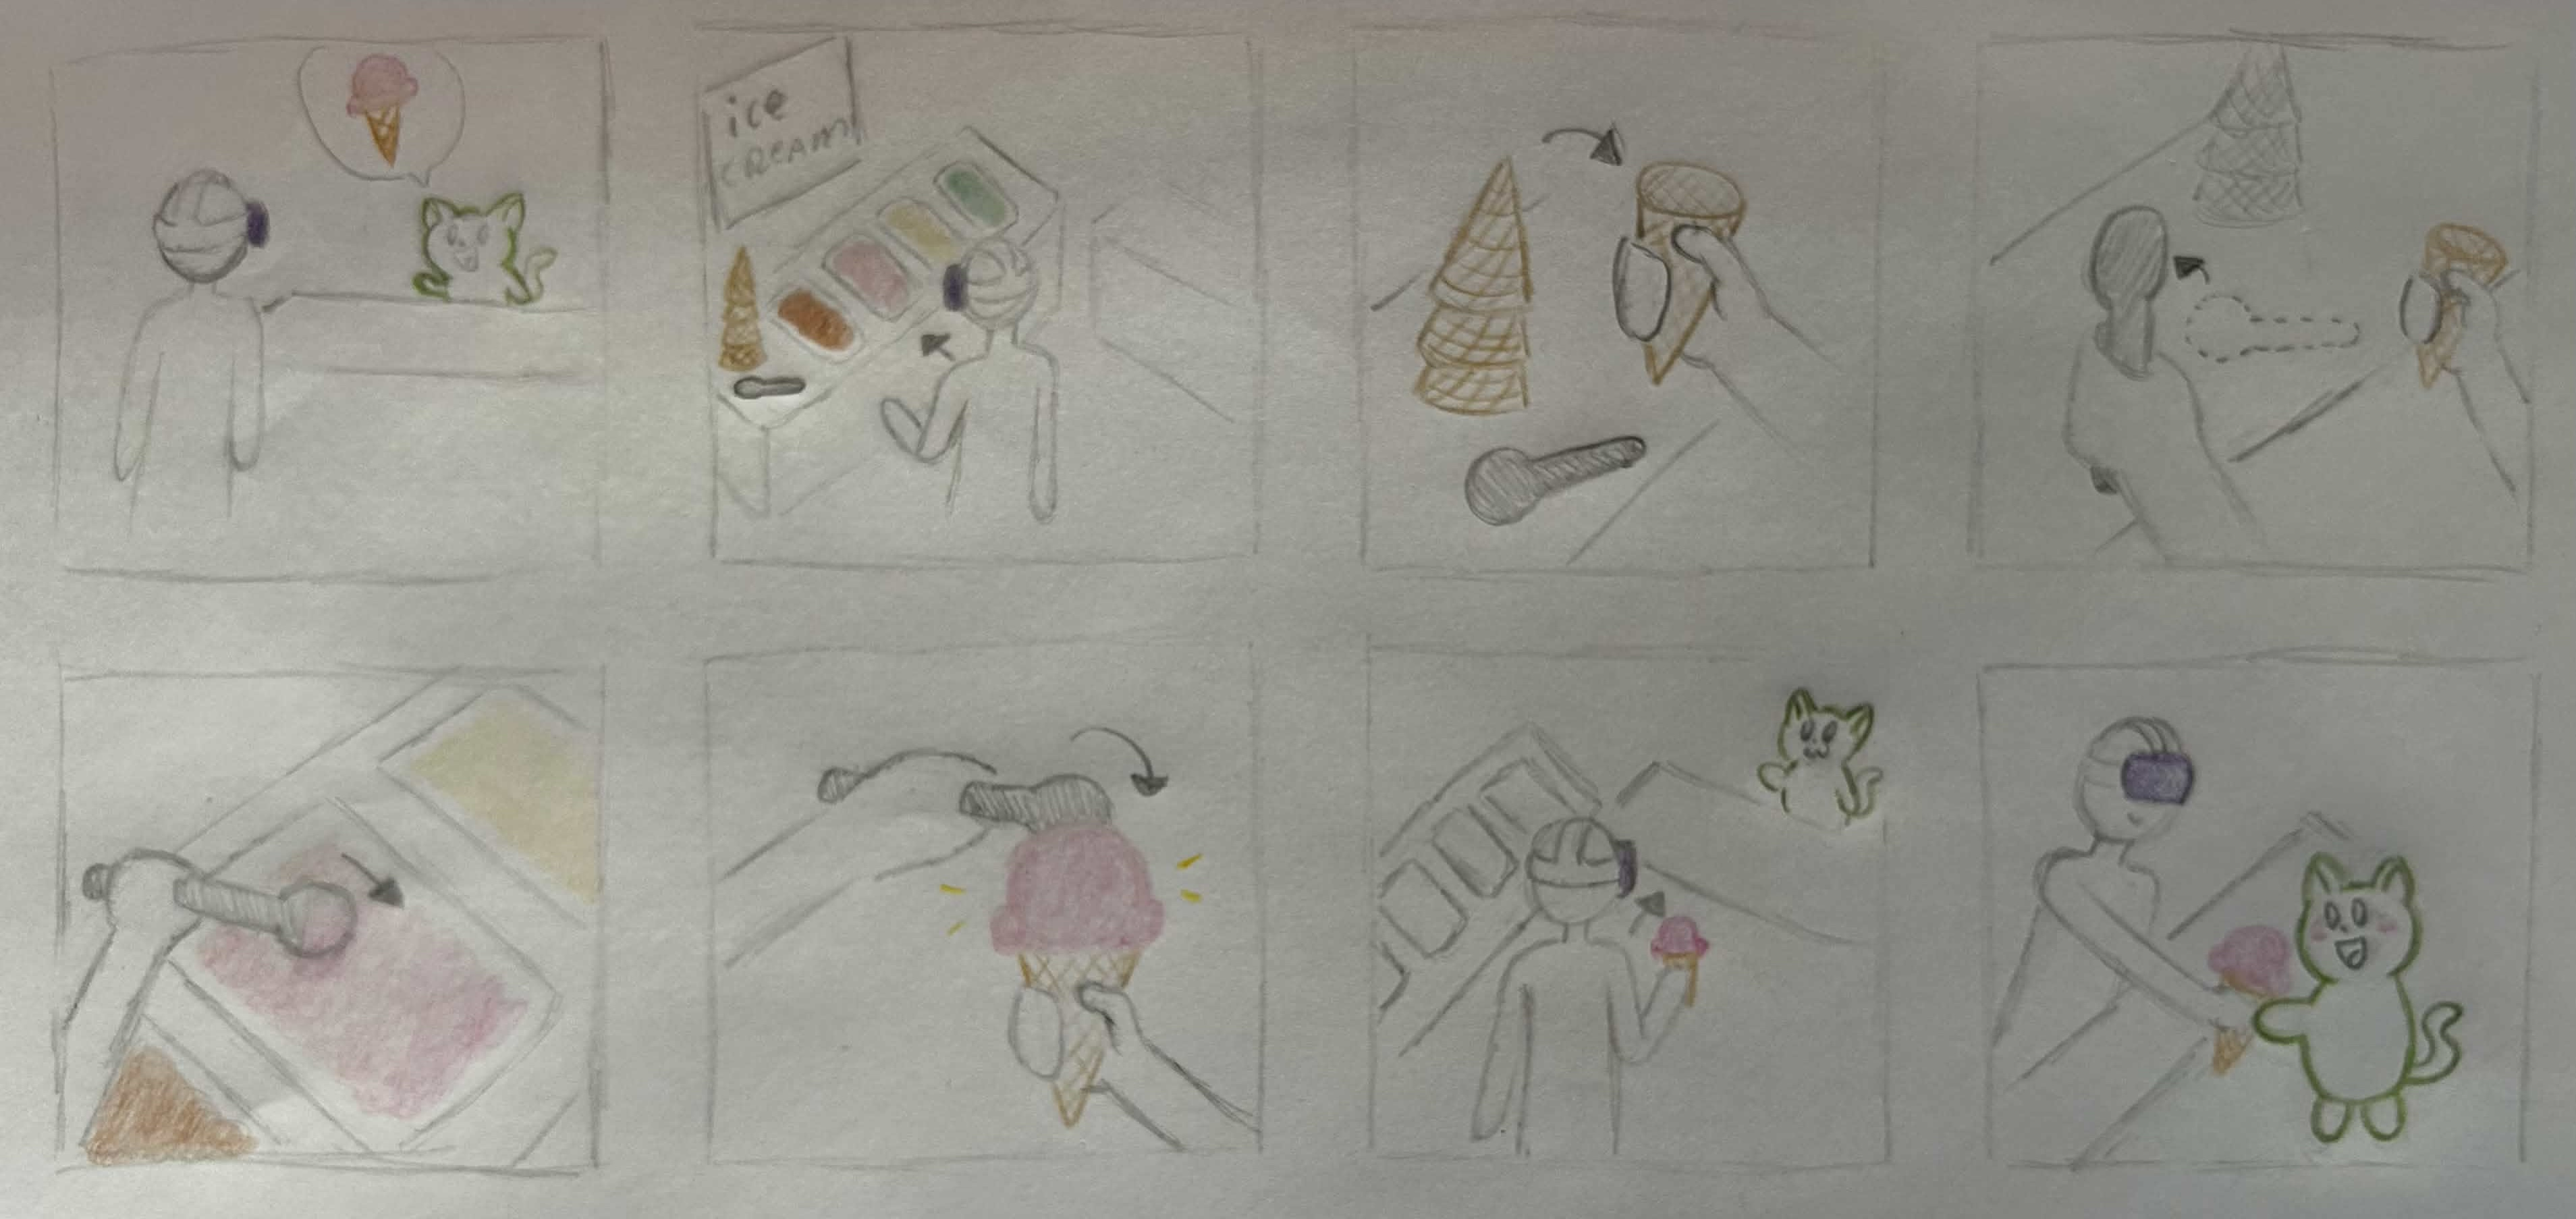
\includegraphics[width=0.4\textwidth]{Imagenes/Storyboard.jpg}}
\caption{Storyboard de una interacción planificada para \textit{Cozyffee VR}}
\label{storyboard}
\end{figure}

La figura \ref{storyboard} representa una situación típica de juego en la que el usuario recibe una orden de un cliente, va a una de las estaciones de la cocina a prepararla mediante acciones físicas y luego se la entrega al cliente lista.

\section{Plan de trabajo}

Para el desarrollo del video juego se planea dedicar el primer mes al diseño de interacciones y gameplay loop, el segundo mes al desarrollo del prototipo lofi (es decir, sin animaciones, interacciones básicas, etc.), y para el tercer mes el desarrollo del prototipo hifi (donde se incluirán animaciones e interacciones fuera del gameplay loop principal).\medskip

En la tabla \ref{fechasclave} se detallan algunas fechas límites que se considerarán importantes durante el desarrollo.

\begin{table}[htbp]
    \caption{Fechas clave}
    \begin{center}
        \begin{tabular}{|c|c|}\hline
            \textbf{Actividad} & \textbf{Fecha límite} \\\hline
            Diseño gameplay loop & 22-09-2026 \\\hline
            Testeo con usuarios & 09-10-2026 \\\hline
            Prototipo lo-fi & 12-10-2026 \\\hline
            Diseño UI final & 04-11-2026 \\\hline
            Sistema de progresión & 10-11-2026 \\\hline
            Playtesting & 21-11-2026 \\\hline
            Prototipo hi-fi & 23-11-2026 \\\hline
        \end{tabular}
        \label{fechasclave}
    \end{center}
\end{table}

Dentro de los anexos de este documento es posible encontrar una planificación más detallada en formato de carta Gantt.

\printbibliography

\newpage

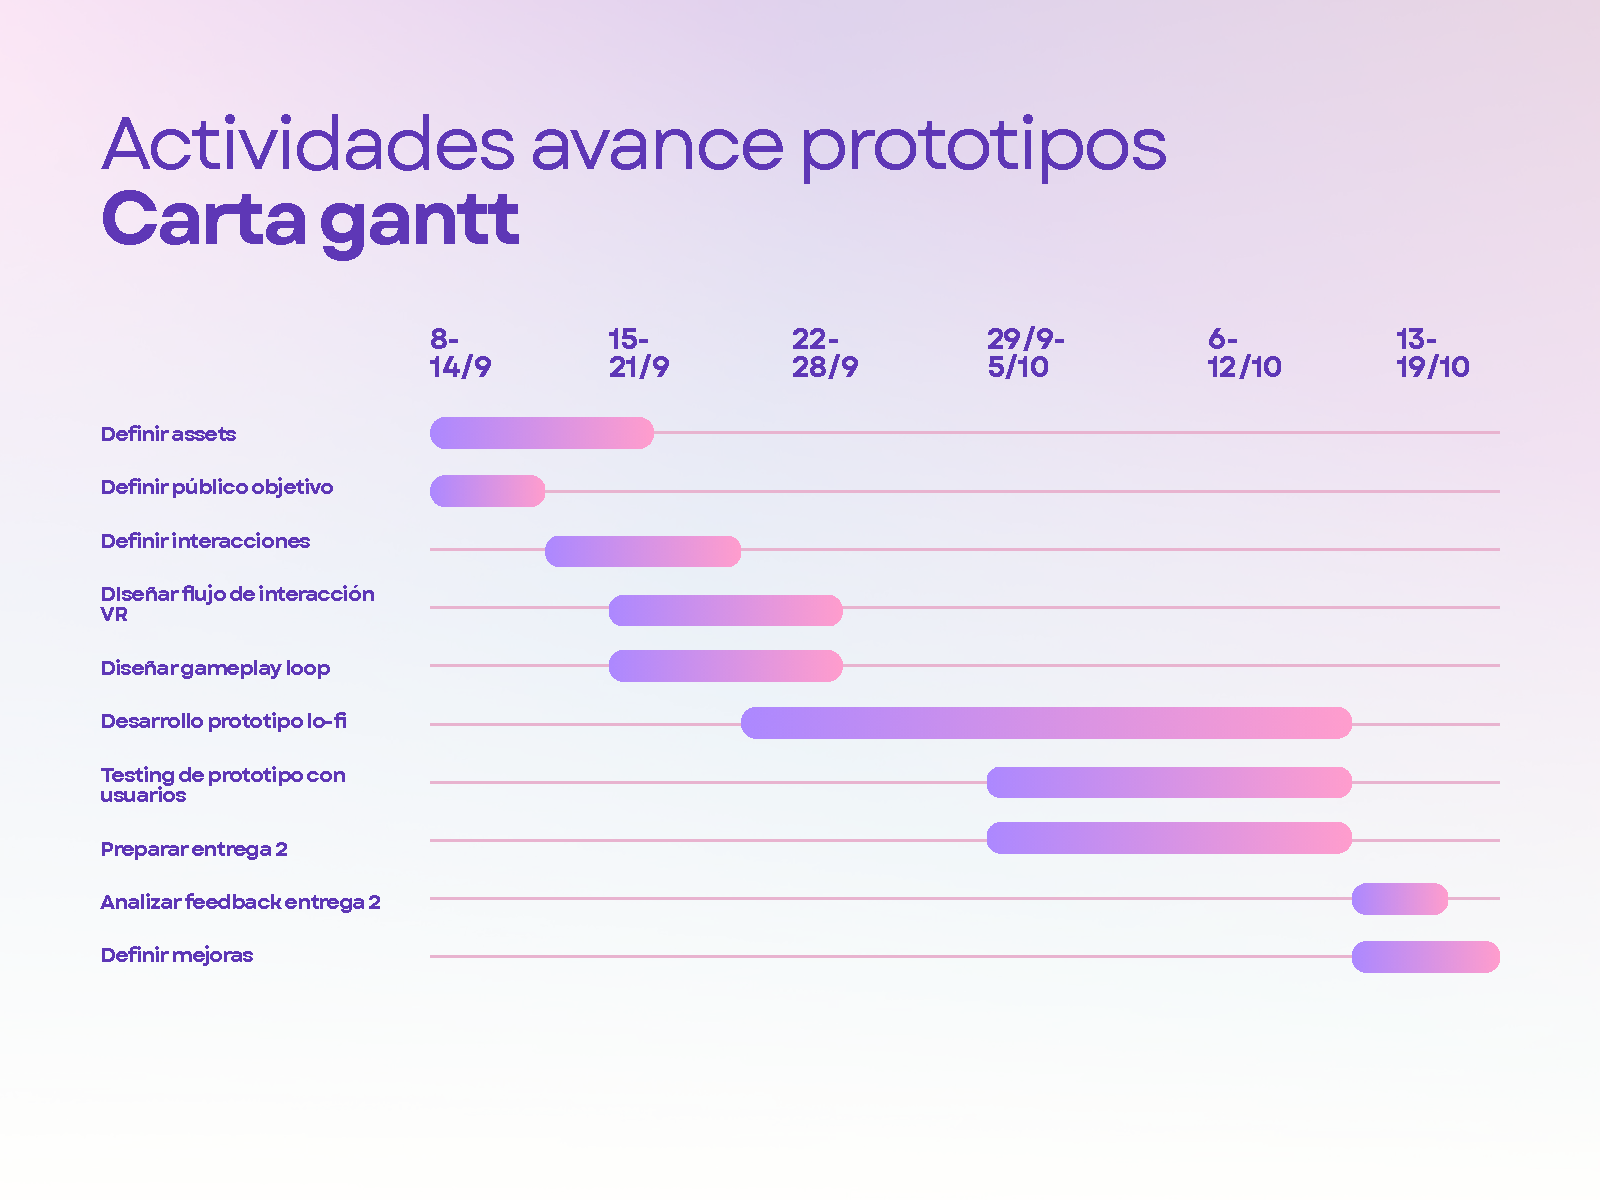
\includepdf[pages=-]{Anexos/Carta_gantt.pdf}

\end{document}
